\subsection{Reguladores de voltaje}

El sistema emplea dos reguladores DC-DC step-down para adaptar la tensión de alimentación principal (24V DC) a los niveles requeridos por diferentes subsistemas:

\underline{Regulador 24V - 5V:} Regulador conmutado step-down con capacidad de 5 A. Este regulador alimenta:
\begin{itemize}[label=$\bullet$]
\item Arduino Mega 2560 (consumo típico 0.5 A)
\item Raspberry Pi 5 (consumo típico 3 A, picos de 4 A)
\item Cámara USB (consumo 0.5 A)
\item Margen de seguridad: 1 A adicional
\end{itemize}

La capacidad total requerida es de 5 A, considerando operación simultánea de todos los dispositivos a carga máxima. El regulador seleccionado proporciona exactamente esta capacidad con margen de seguridad del 20\%.

\underline{Regulador 24V - 12V:} Regulador conmutado step-down con capacidad de 10 A. Este regulador alimenta:
\begin{itemize}[label=$\bullet$]
    \item Dos servomotores Dynamixel MX-106T/R (consumo máximo de 4.8 A cada uno)
    \item Circuitos lógicos de drivers de motores (aproximadamente 100 mA por driver)
\end{itemize} 
Considerando un escenario de operación simultánea bajo carga, se estima un consumo total de 6-7 A, dejando margen de seguridad del 30-40\% para picos transitorios.

La separación de la alimentación lógica de los drivers respecto a la alimentación de procesadores (5V) previene caídas de tensión causadas por conmutación de alta frecuencia que podrían inducir resets espurios del Arduino.

La Figura \ref{fig:diagrama_voltajes} ilustra el esquema completo de distribución de voltajes desde la fuente primaria de 24V hasta todos los componentes del sistema.

\begin{figure}[H]
\centering
% TODO: Agregar imagen del diagrama de distribución de voltajes
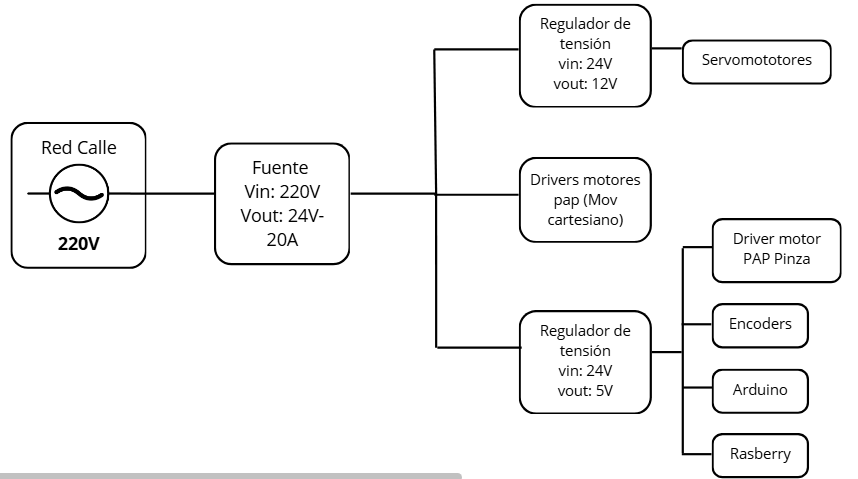
\includegraphics[width=0.75\textwidth]{img/diagrama_voltajes_real.png}
\caption{\textit{Diagrama de distribución de voltajes del sistema mostrando fuente de 24V, reguladores step-down (24V→5V y 24V→12V), y conexiones a todos los componentes}}
\label{fig:diagrama_voltajes}
\end{figure}
